\documentclass[Softwaredesign/Softwaredesign_main.tex]{subfiles}
\begin{document}
\subsection{Design af GameController (Playerside)}\label{sec:GameController_design_bilag}
GameController klassen sørger for logikken for PlayerSideApp. Den skal sørge for at de tre boundary klasser RPI\_IF, CupLight\_IF og CupSensor\_IF kan spille sammen og få PlayerSideApp til at fungerer, som den skal. Da denne klasse blev lavet var det meget vigtigt at følge sekvensdiagrammet i software arkitekturen for PlayerSideApp, da de funktioner, der bruges er brugt af de forskellige boundary klasser. Der er også lavet stubs til de metoder, som hører til de tre boundary klasser, hvor der bare bliver udskrevet de nødvendige information for de forskellige metoder, så man er sikker på de er kaldt med de rigtige værdier. Disse stubs består udelukkende af udskrivning til terminalen. Udover kun at gøre dette i stubs funktionerne, så er det også gjort for de fleste funktioner i gamecontroller klassen. Alt dette er gjort så det bliver utrolig let at debugge problemer, der skulle opstå i både modultest, men senere også integrationstest af hele PlayerSideApp. Til dette er komponenten UART[v2.50] brugt i PSoC's komponentkatalog og er utrolig let at sætte op til dette formål. Da man bare skal kalde funktionen UART\_Start efter at have indsat komponenten i PSoC creators design side, hvorefter man kan lave en buffer med funktionen sprintf, som man bruger som argument i funktionen UART\_PutString(). 
\subsubsection{States og variabler}
For at få et bedre overblik over denne klasse er det en god ide at forstå de variabler og states klassen arbejder på.
\textbf{Enum Gamestate}
Gamestate er en enum i GameController klassen som beskriver alle de states klassen kan være i. De fem states er: IDLE, STARTING, PLAYING, WON og LOST. Kun i metoden setState kan disse ændres efter en besked er sendt fra raspberry pie.
\textbf{myColor og opponentColor}
De to variabler er af typen color\_t, som er beskrevet i Cup\_Light\_IF's design. De er til for at holde henholdsvis holde sin egen farve samt modstanderens farve. De opdateres med metoderne setMyColor og setOpponentColor. Disse metoder bliver kaldt i RPI\_IF's metode RPI\_IF\_handledata i tilfældet, hvor en farvekode besked bliver sendt til PSoC'en. 
\textbf{CupStatus}
Denne variabel er af typen uint8\_t. Denne variabel opdateres af metoden updateCupStatus, som kaldes fra CupSensor\_IF klassen, når en kop bliver fjernet eller placeret på en af de 6 kopholdere. De 6 mindst betydende bits svarer til status for en kopholder. Når et bit er sat er en kop placeret på den tilsvarende kopholder. Hvis den er lav er en kop ikke placeret på den tilsvarende kopholder. 
\textbf{HitStatus}
Denne variabel er af typen uint8\_t Hver gang en kop er ramt vil denne variabel opdateres. Dette sker ved, at CupSensor\_IF klassen kalder updateHitStatus metoden. Her er fungerer det på samme måde måde, som med CupStatus variablen. Hver af de 6 mindst betydende bits vil have en kopholder associeret med sig(den samme som Cupstatus). En sat bit værdi svarer til at en kop er ramt og ikke løftet ellers er den lav. Når en bit er sat vil metoden controller sørge for at det associerede lys for kopholderen blinker. Dette uddybes mere, når denne metode forklares længere nede.
\textbf{placedCupColor, missingCupColor og turnedOffColor}
Disse 3 variabler er alle et struct af typen color\_t. De har alle en fast farvekode(color\_t beskriver farvekoden) i systemet. TurnedOffColor bruges, når systemets state bliver sat til IDLE, hvor funktionen ControlLight i CupLight\_IF bliver kaldt med denne varibale som argument, hvorved alle kopholder lysene slukkes. PlacedCupColor og missingCupColor bliver begge brugt i funktionen controlLights, når systemet er i state STARTING. Her skal disse to farver lyse istedet for MyColor og opponentColor.
\textbf{Blinking}
Når Nogle af bits i Hitstatus er sat og systemet er i state PLAYING, så skal en eller flere(afhængig af HitStatus variablen) blinke. Her har vi en blinking variabel som er 1, når hit status er andet end 0 og 0, når hit status er 0. Denne variabel er inkluderet, så timeren, der styrer blink ikke er konstant skaber et interrupt.
\subsubsection{Metoder i Gamecontroller}
\textbf{Controller}\\
Denne metode bliver kaldt i det uendelige for loop i main. Den starter med et if statement, der bliver kørt hvis systemet er i STARTING eller PLAYING. Endnu et if statemet ser på om CupStatus har ændret sig. Hvis den er ændret vil funktionen ControlLights kaldes med den nye CupStatus som argument. Den styrer så de forskellig kopholder lys. Udover dette styrer metoden også om nogle af kop holder lysene skal blinke ved at styrer timeren. Dette gøres i et if statement, hvor der ses på om systemet er i state PLAYING. Hvis det er sandt vil en timer startes, hvis hitstatus er andet end 0 og timeren ikke allerede er startet(blinking er 0). Derimod vil timeren stoppes, hvis hitstatus er 0 og timeren er igang(blinking er 1).
\textbf{setState}\\
Denne metode kaldes i RPI\_IF hver gang, der sendes en besked til PSoC fra rpi med hex værdierne 0x0A til 0x0E. Her vil der i argumentet blive brugt en af de 5 enums af typen Gamestate. Metoden består af et switch statement, hvor hver state har forskellige funktioner for det første bliver currentState ændret til den sendte state i alle casene. Udover dette vil, der i case IDLE blive kaldt funktionen ControlAllLights i CupLight\_IF med variablen turnedOffColor som argument. I case STARTING vil getCupstatus kaldes i CupSensor\_IF, hvor den Cupstatus opdateres ud fra retur værdien. Denne Cupstatus sendes videre til RPI med RPI\_IF's sendCupStatus funktion og ControlLights bliver kaldt med Cupstatus som argument. Det samme gøres i case PLAYING. I case WON bliver ControlAllLights kaldt med MyColor som argument. I case LOST bliver den samme metode kaldt som i case WON, men med opponentColor som argument.
\textbf{interrupt\_blink}\\
Denne funktionen bliver kun kaldt i timerens interruptvektor. Hvis systemet er i state PLAYING, så vil et loop på 8 køres igennem, som ser på de forskellige bits i Hitstatus, hvis et bit er sat vil det pågældende bit nummer slået op i et array som holder blink status for den pågældende kopholder alt afhængig af om værdien er 0 eller 1 vil controlLight i CupLight\_IF kaldes med index(samme som bit nummer) og enten opponentColor(når værdien på index er 0) eller myColor(når værdien på index er 1).
\textbf{updateCupStatus}\\
Denne funktion kaldes af CupSensor klassen, når CupStatus skal opdateres(når en kop placeres eller fjernes fra kop holder). Der ses først på om systemet er i state STARTING eller PLAYING. I dette tilfælde opdateres CupStatus til det, der er sendt med som argument til metoden. Herefter sendes den opdaterede cup 
status til RPI med metoden sendCupStatus i RPI\_IF klassen. 
\textbf{updateHitStatus}\\
Denne metode blive givet den nuværende hit status fra CupSensor klassen, og hvis systemet er i state PLAYING, så vil variablen updateHitStatus opdateres. Det er metoden Controller, der skal håndterer, denne ændring.
\textbf{ControlLights}\\
Denne metode modtager Cupstatus som argument. Hvis systemet er i state STARTING, så vil et loop køres igennem otte gange, hvor alle bits i et uint8\_t array(blink status for de enkelte LED'er), checkes igennem for om det er højt eller lavt. Hvis det er 1 vil controllight metoden kaldes med index og placedCupColor, hvorimod den kaldes med index og missingCupColor, hvis det er 0. Når Systemet er i state PLAYING, så vil det samme gøres, som i state STARTING, bortset fra at istedet for placedCupColor vil MyColor sendes med som argument i metoden controllight, og opponentColor vil sendes med istedet for missingCupColor.
\subsubsection{Komponenter}
Den eneste komponent brugt i denne klasse udover UART er en timer, som er en del af PSoC creator komponentkatalog. Komponenten kan ses i figur \ref{fig:Timer}.
\begin{figure}
    \centering 
    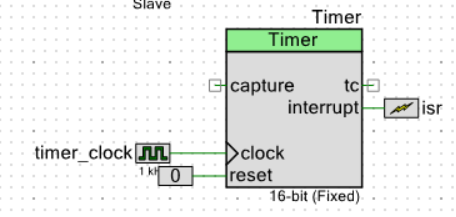
\includegraphics[width=\linewidth]{Softwaredesign/GameController/graphic/gamecontroller_timer.PNG}
    \caption{Timer brugt til blinke funktionen i GameController klassen.}
    \label{fig:Timer}
\end{figure}
Komponenten initieres i main ved at kalde Timer\_Start(). Den er i konstant run mode, hvilket vil sige, at når den først startes så stoppes den ikke før funktionen Timer\_Stop() kaldes. Den startes ved at kalde Timer\_Start() og vil herefter interrupte hvert halve sekund, hvilket er den periode den er indstillet til. Inde i Interrupt vektoren bliver funktionen Timer\_ReadStatusRegister kaldt, hvilket er nødvendigt for at timeren køre indtil den stoppes. Dette var nødvendigt, da TC bit i timerens status register  ellers ville forblive højt, og dermed ville den ikke interrupte mere end en gang. Start og stop af timeren kontrolleres i Controller funktionen. Den eneste funktion, der kaldes i interrupt vektoren er metoden interrupt\_blink. I figur \ref{fig:Timer_setting} ses timerens konfiguering.
\begin{figure}
    \centering 
    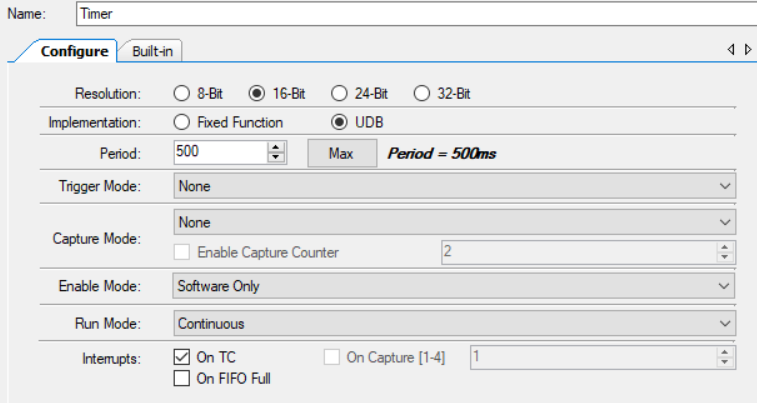
\includegraphics[width=\linewidth]{Softwaredesign/GameController/graphic/timer_settings.PNG}
    \caption{Timer konfiguering.}
    \label{fig:Timer_setting}
\end{figure}
\end{document}